
Having written a completely general program, we are free to add as many
celestial objects as we'd like. However, we start by looking at the Sun-Earth
system in order to test the stability of our program as function of time step
$dt$.

Having approximated Earth's orbit around the Sun as circular, we obtained our
mass units. We apply Newton's 2nd law and his gravitational law to find at which
velocity the orbit is circular, $M_E$ being the Earth's mass.
%
\begin{align*}
	F_G &= M_{\text{E}}a \\
	G \frac{M_{\odot}M_{\text{E}}}{r^2} &= M_{\text{E}}a
\end{align*}
%
For circular orbits we can write the acceleration as
%
\begin{equation*}
	a = \frac{v^2}{r}
\end{equation*}
which gives us
%
\begin{align*}
	v^2 &= G \frac{M_{\odot}}{r^2} \\
	v &= \sqrt{ \frac{GM_{\odot}}{r^2}}
\end{align*}
%
Inserting $GM_{\odot} = 4\pi^2$, $r = 1$ AU, we get
%
\begin{equation*}
	v = 2\pi
\end{equation*}
%
We place the Sun at the origin, with Earth at a distance 1 AU in $x$-direction.
Earth's velocity $v$ is initially directed in the $y$-direction. The orbit
around the Sun is shown in \refig{sunEarth-dt0.01}.
%
% \begin{figure}[htpb]
	% \centering
	% 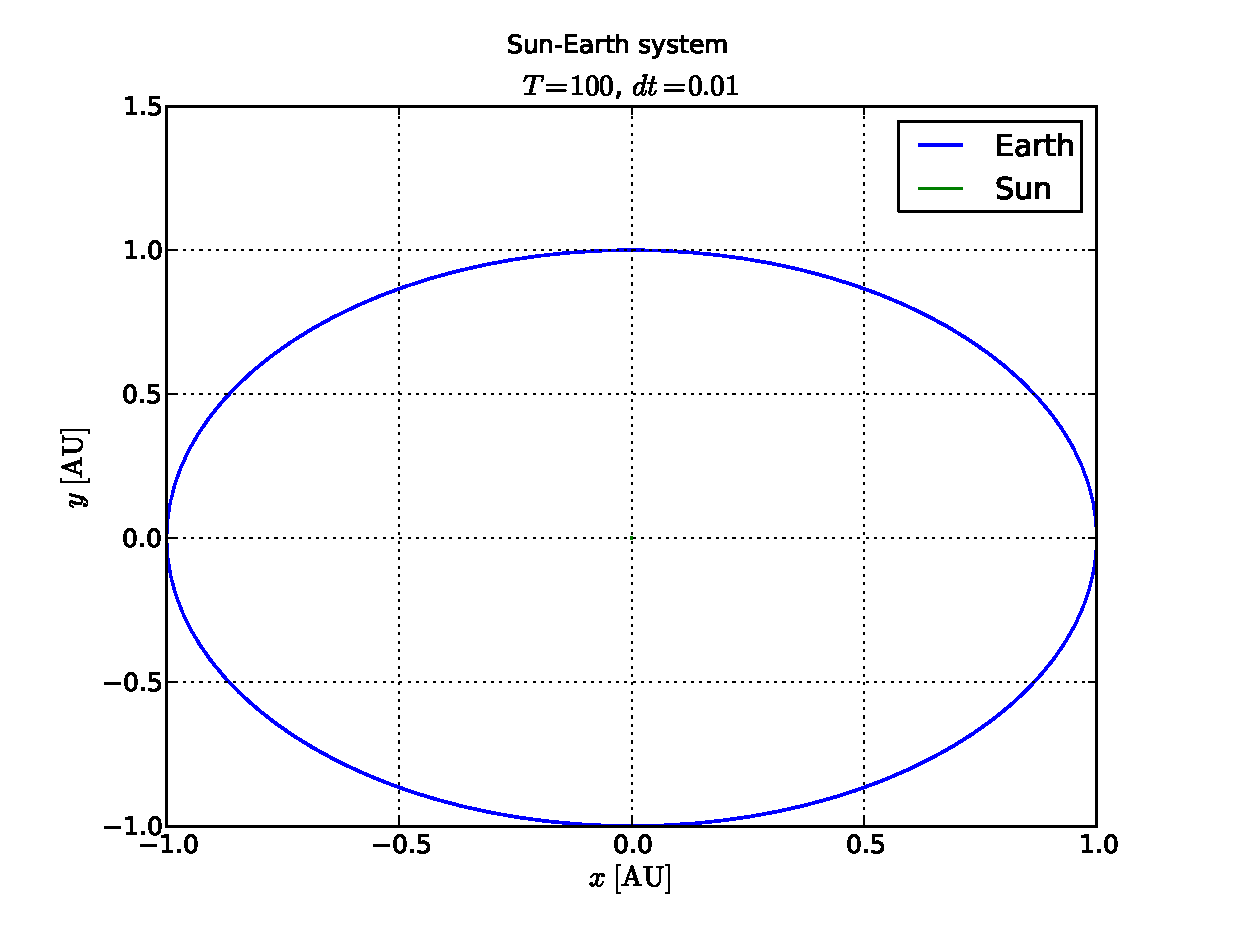
\includegraphics[width=1.0\textwidth]{../../results/sun_earth_T100_dt1e-2}
	% \caption{Earth's circular orbit around the Sun over a period of $T = 100$
		% years, with time step $dt = 0.01$. The initial position was
		% $\mathbf{r} = [1,0]$, $\mathbf{v} = [0,1]$.}
	% \label{fig:sunEarth-dt0.01}
% \end{figure}
%
